	\newpage

\section{Diagram pzypadków użycia}

\begin{figure}[H]
	\centering
	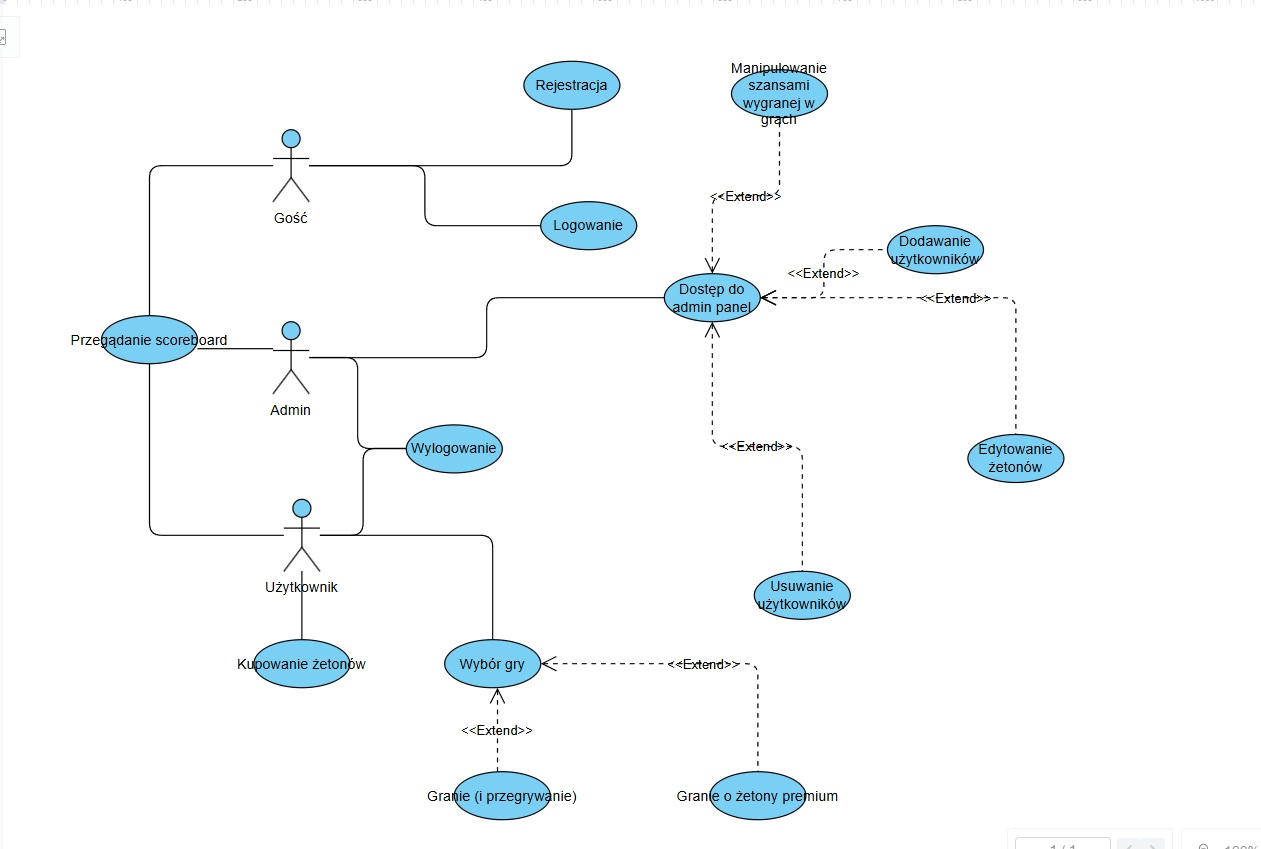
\includegraphics[width=1\textwidth]{images/przypadki_uzycia.png}
	\caption{\centering{Diagram przypadków użycia}}
\end{figure}

\section{Scenariusze}

\begin{itemize}
  \item Logowanie
  \begin{itemize}
    \item Gość wchodzi na stronę główną i klika przycisk "Zaloguj się".
    \item Pojawia się strona logowania i gość wpisuje swój email oraz hasło.
    \item Wynik:
    \begin{itemize}
      \item Logowanie z danymi użytkownika: Gość zostaje przeniesiony na sesję użytkownikową oraz zostaje przeniesiony na główną stronę aplikacji.
      \item Logowanie z danymi administratora: Gość zostaje przeniesiony na sesję administratora oraz zostaje przeniesiony na główną stronę aplikacji.
    \end{itemize}
    \item Wynik alternatywny:
    \begin{itemize}
      \item Gość wpisuje niepoprawne dane: Pojawia się komunikat, że email i hasło są niepoprawne. Gość pozostaje na stronie logowania.
    \end{itemize}
  \end{itemize}
  \item Rejestracja
  \begin{itemize}
    \item Gość wchodzi na stronę główną i klika przycisk "Zarejestruj się".
    \item Pojawia się okno rejestracji. Użytkownik podaje swój email, nazwę, hasło i powtórkę hasła.
    \item Wynik:
    \begin{itemize}
      \item Poprawnie zformatowane dane logowania: Zostaje stworzone nowe konto oraz gość zostanie przeniesiony na sesję użytkownika.
    \end{itemize}
    \item Wynik alternatywny:
    \begin{itemize}
      \item Niepoprawne zformatowane dane logowania: Pojawia się komunikat o niepoprawnie zformatowanych danych rejestracji i użytkownik pozostaje na stronie rejestracji.
      \item Hasła się nie zgadzają: Pojawia się komunikat, że hasła się nie zgadzają. Pola z hasłami są resetowane.
    \end{itemize}
  \end{itemize}
\end{itemize}
